\section{Bottom Class Reference}
\label{classBottom}\index{Bottom@{Bottom}}
{\tt \#include $<$bottom.h$>$}

Inheritance diagram for Bottom:\begin{figure}[H]
\begin{center}
\leavevmode
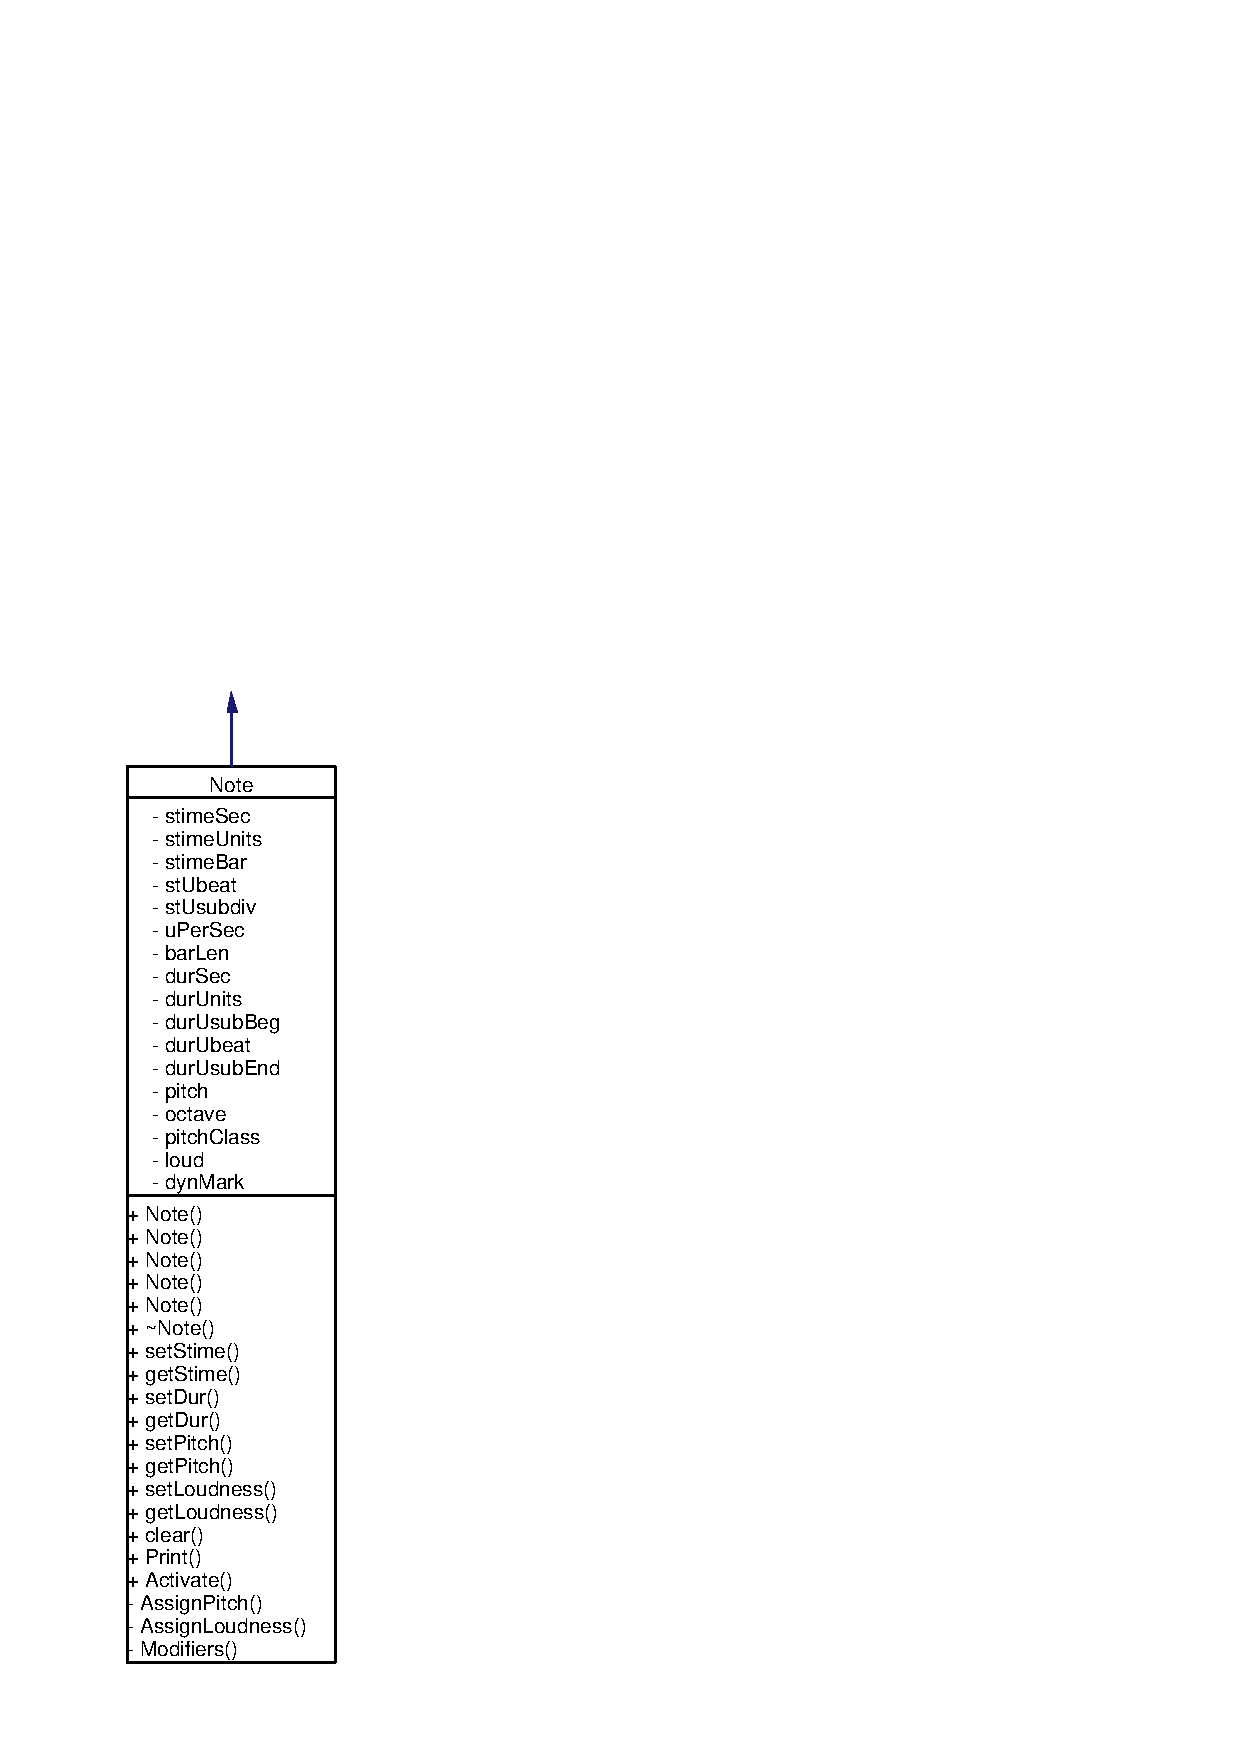
\includegraphics[width=93pt]{classBottom__inherit__graph}
\end{center}
\end{figure}
Collaboration diagram for Bottom:\begin{figure}[H]
\begin{center}
\leavevmode
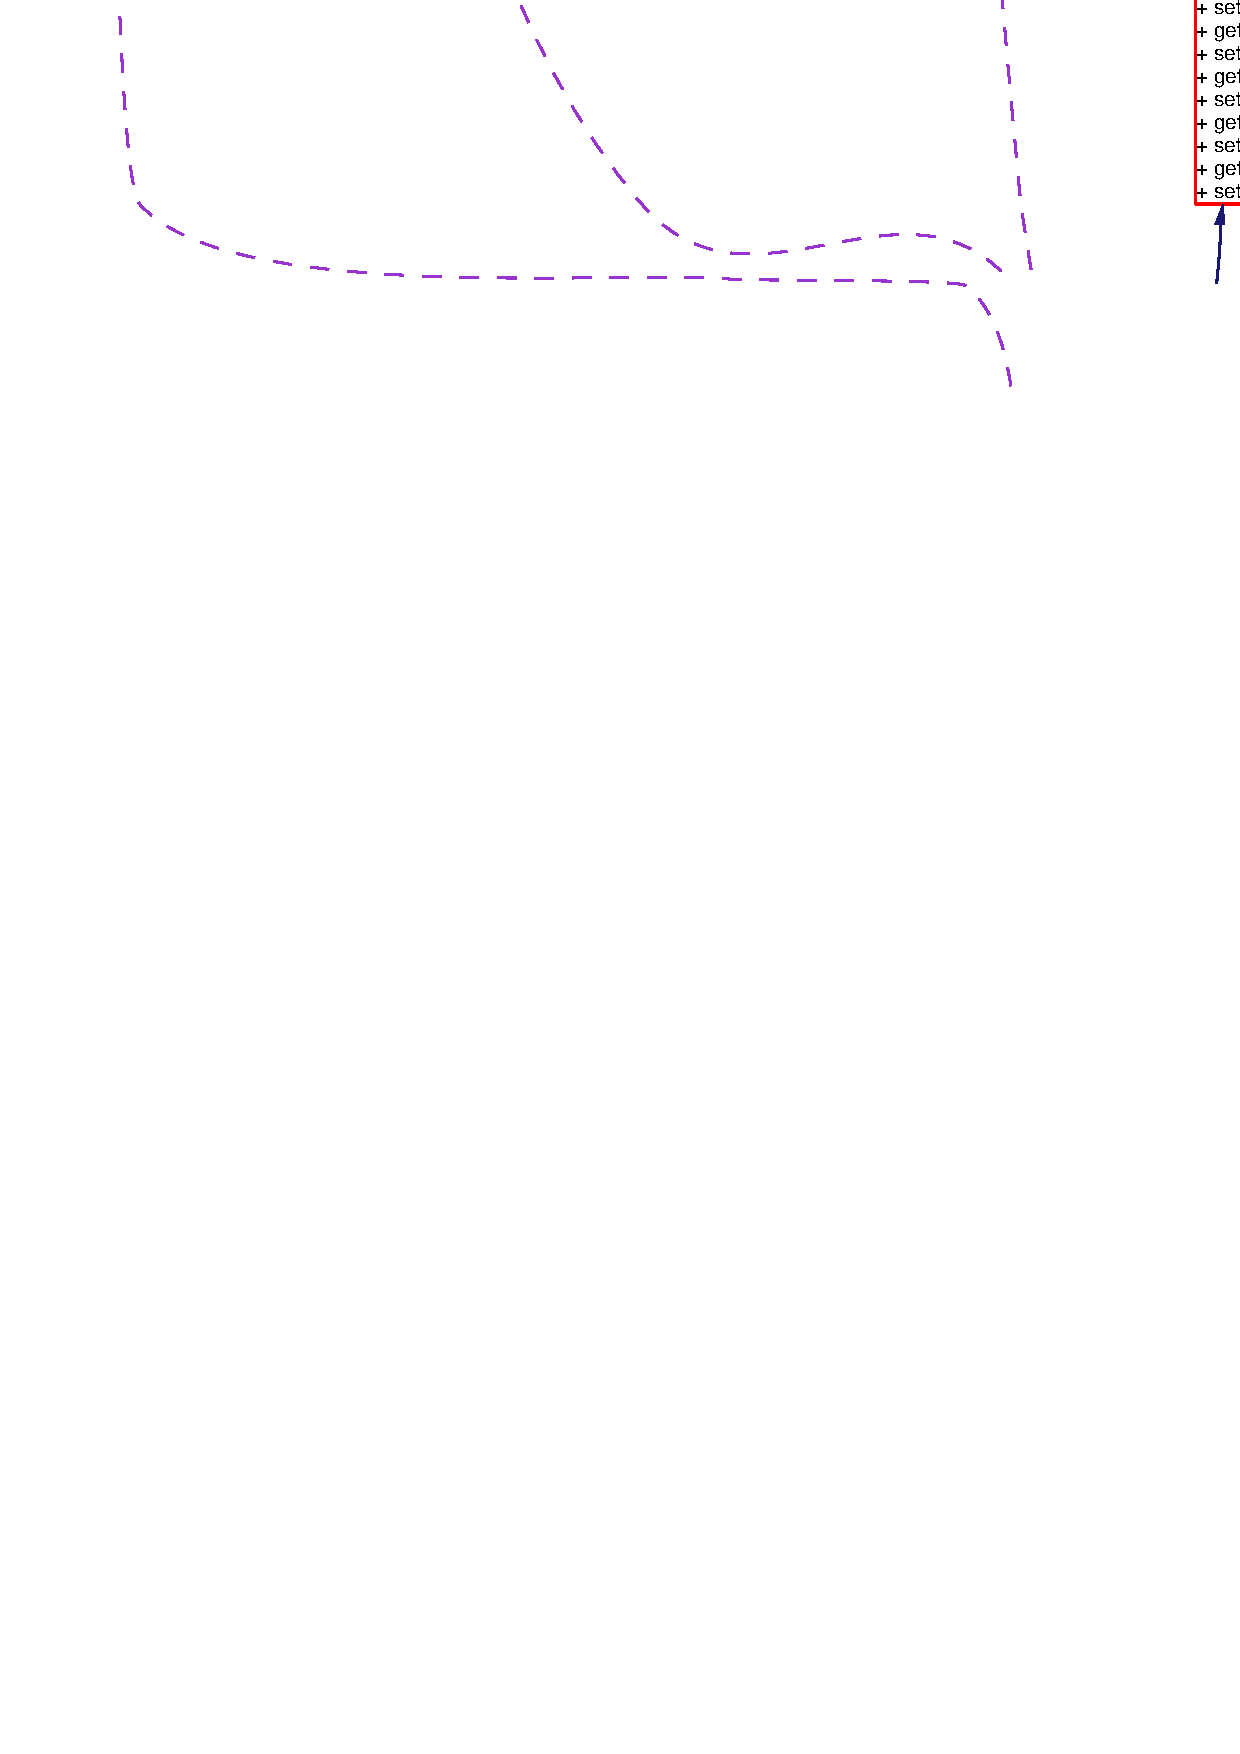
\includegraphics[width=420pt]{classBottom__coll__graph}
\end{center}
\end{figure}
\subsection*{Public Member Functions}
\begin{CompactItemize}
\item 
{\bf Bottom} ()
\item 
{\bf Bottom} (float astart\-Time, float a\-Duration, int a\-Type, char $\ast${\bf a\-Name})
\item 
{\bf Bottom} (const  {\bf Bottom} \&orig\-Bottom)
\item 
{\bf $\sim$Bottom} ()
\item 
{\bf Bottom} \& {\bf operator=} (const  {\bf Bottom} \&orig\-Bottom)
\item 
void {\bf clear} ()
\item 
void {\bf set\-Name} (char $\ast${\bf a\-Name})
\item 
virtual void {\bf set\-Start\-Time} (float a\-Start\-Time)
\item 
virtual void {\bf set\-Duration} (float a\-Duration)
\item 
void {\bf set\-Density} (double a\-Density)
\item 
void {\bf set\-Num\-Partials} (int a\-Num\-Partials)
\item 
void {\bf Create\-New\-Objects} ()
\item 
void {\bf Implement} ()
\item 
void {\bf build\-Sound} (Score $\ast${\bf score})
\item 
float {\bf Assign\-Freq} (double {\bf check\-Point})
\item 
int {\bf Num\-Part} (float freq)
\item 
int {\bf Spectrum} (Sound $\ast$s, float freq)
\item 
void {\bf Create\-Partials} (Sound $\ast$s, int num\-Partials)
\item 
void {\bf Set\-Frequency} (Sound $\ast$s, float deviation, float base\-Freq, int num\-Partials)
\item 
void {\bf One\-Step} (Sound $\ast$s, double {\bf check\-Point}, int num\-Partials)
\item 
void {\bf Three\-Step} (Sound $\ast$s, double {\bf check\-Point}, int num\-Partials)
\item 
void {\bf Rules} (int num\-Partials, float amp\-Scale[$\,$])
\item 
float {\bf Loud} (Sound $\ast$s, double {\bf check\-Point})
\item 
void {\bf Modifiers} (Sound $\ast$s, int num\-Partials, double {\bf check\-Point})
\item 
void {\bf Choose\-Sound\-Dyn\-Param} (Sound $\ast$s, const  char $\ast$modifier, Envelope $\ast$env)
\item 
void {\bf Choose\-Partial\-Dyn\-Param} (Sound $\ast$s, const  char $\ast$modifier, Envelope $\ast$env, int i)
\item 
void {\bf Spatialization} (Sound $\ast$s, double {\bf check\-Point})
\item 
void {\bf Spatialization} (Sound $\ast$s, double {\bf check\-Point}, string method, Envelope $\ast$chance, Envelope $\ast$pan)
\item 
void {\bf Reverberation} (Sound $\ast$s, double {\bf check\-Point})
\item 
void {\bf Reverberation} (Sound $\ast$s, double {\bf check\-Point}, string method, Envelope $\ast$chance, float room\-Size)
\item 
void {\bf Print} ()
\item 
void {\bf Print\-Sound} (int num\-Partials, float freq, float sones)
\item 
virtual void {\bf build\-Note} ()
\end{CompactItemize}
\subsection*{Public Attributes}
\begin{CompactItemize}
\item 
{\bf File\-Value} $\ast$ {\bf bottom\_\-new\-Object\-Method}
\item 
{\bf File\-Value} $\ast$ {\bf bottom\_\-slope}
\item 
{\bf File\-Value} $\ast$ {\bf bottom\_\-freq\-Method}
\item 
{\bf File\-Value} $\ast$ {\bf bottom\_\-freq\-Method2}
\item 
{\bf File\-Value} $\ast$ {\bf bottom\_\-abs\-Range}
\item 
{\bf File\-Value} $\ast$ {\bf bottom\_\-pat\-File}
\item 
{\bf File\-Value} $\ast$ {\bf bottom\_\-fundamental}
\item 
{\bf File\-Value} $\ast$ {\bf bottom\_\-sound\-Method}
\item 
{\bf File\-Value} $\ast$ {\bf bottom\_\-env\-Method}
\item 
{\bf File\-Value} $\ast$ {\bf bottom\_\-amp\-Method}
\item 
{\bf File\-Value} $\ast$ {\bf bottom\_\-rule}
\item 
{\bf File\-Value} $\ast$ {\bf bottom\_\-rand\-Flag}
\item 
{\bf File\-Value} $\ast$ {\bf bottom\_\-amp\-Scale}
\item 
{\bf File\-Value} $\ast$ {\bf bottom\_\-factor}
\item 
{\bf File\-Value} $\ast$ {\bf bottom\_\-attenuation}
\item 
{\bf File\-Value} $\ast$ {\bf bottom\_\-modifier}
\item 
{\bf File\-Value} $\ast$ {\bf bottom\_\-select}
\item 
{\bf File\-Value} $\ast$ {\bf bottom\_\-spat\-Method}
\item 
{\bf File\-Value} $\ast$ {\bf bottom\_\-reverb\-Method}
\end{CompactItemize}
\subsection*{Protected Attributes}
\begin{CompactItemize}
\item 
char $\ast$ {\bf bottom\-Name}
\item 
float {\bf bottom\-Start\-Time}
\item 
float {\bf bottom\-Duration}
\item 
int {\bf bottom\-Type}
\item 
int {\bf bottom\-Num\-Partials}
\end{CompactItemize}
\subsection*{Private Attributes}
\begin{CompactItemize}
\item 
double {\bf bottom\-Density}
\end{CompactItemize}


\subsection{Detailed Description}
This class is used to store and manage the details of a bottom event. 



Definition at line 50 of file bottom.h.

\subsection{Constructor \& Destructor Documentation}
\index{Bottom@{Bottom}!Bottom@{Bottom}}
\index{Bottom@{Bottom}!Bottom@{Bottom}}
\subsubsection{\setlength{\rightskip}{0pt plus 5cm}Bottom::Bottom ()\hspace{0.3cm}{\tt  [inline]}}\label{classBottom_a0}




Definition at line 63 of file bottom.h.\index{Bottom@{Bottom}!Bottom@{Bottom}}
\index{Bottom@{Bottom}!Bottom@{Bottom}}
\subsubsection{\setlength{\rightskip}{0pt plus 5cm}Bottom::Bottom (float {\em astart\-Time}, float {\em a\-Duration}, int {\em a\-Type}, char $\ast$ {\em a\-Name})}\label{classBottom_a1}


This is a constructor. \begin{Desc}
\item[Parameters:]
\begin{description}
\item[{\em astart\-Time}]The start time of the event \item[{\em a\-Duration}]The duration of the event \item[{\em a\-Type}]The type of the event \item[{\em a\-Name}]A name for the event \end{description}
\end{Desc}
\begin{Desc}
\item[Returns:]A Bottom object \end{Desc}


Definition at line 39 of file bottom.cpp.

References Event::a\-Name, bottom\-ID, bottom\-Type, set\-Density(), set\-Duration(), set\-Name(), and set\-Start\-Time().

Here is the call graph for this function:\begin{figure}[H]
\begin{center}
\leavevmode
\includegraphics[width=144pt]{classBottom_a1_cgraph}
\end{center}
\end{figure}
\index{Bottom@{Bottom}!Bottom@{Bottom}}
\index{Bottom@{Bottom}!Bottom@{Bottom}}
\subsubsection{\setlength{\rightskip}{0pt plus 5cm}Bottom::Bottom (const {\bf Bottom} \& {\em orig\-Bottom})}\label{classBottom_a2}


This is the copy constructor. \begin{Desc}
\item[Parameters:]
\begin{description}
\item[{\em orig\-Bottom}]The Bottom to copy \end{description}
\end{Desc}
\begin{Desc}
\item[Returns:]A copy of orig\-Bottom \end{Desc}


Definition at line 56 of file bottom.cpp.

References bottom\-ID.\index{Bottom@{Bottom}!~Bottom@{$\sim$Bottom}}
\index{~Bottom@{$\sim$Bottom}!Bottom@{Bottom}}
\subsubsection{\setlength{\rightskip}{0pt plus 5cm}Bottom::$\sim${\bf Bottom} ()}\label{classBottom_a3}


This is the destructor. 

Definition at line 65 of file bottom.cpp.

\subsection{Member Function Documentation}
\index{Bottom@{Bottom}!AssignFreq@{AssignFreq}}
\index{AssignFreq@{AssignFreq}!Bottom@{Bottom}}
\subsubsection{\setlength{\rightskip}{0pt plus 5cm}float Bottom::Assign\-Freq (double {\em check\-Point})}\label{classBottom_a14}


This function contains three methods to determine the frequency: FUNDAMENTAL: assumes that each frequency is an \char`\"{}overtone\char`\"{} of a common fundamental, the total duration of the piece WELL\_\-TEMPERED: produces frequencies corresponding to the well-temperate tuning with C0=16.35Hz, the lowest possible frequency CONTINUUM: uses a distribution within a give range

FUNDAMENTAL and WELL\_\-TEMPERED also use a second method selected from: SIEVE: uses a given sieve SEQUENCE: reproduces an ordered sequence of values. The location in the array (offset) can be determined by either the type or the number of the object. \begin{Desc}
\item[Parameters:]
\begin{description}
\item[{\em check\-Point}]\end{description}
\end{Desc}
\begin{Desc}
\item[Returns:]the frequency determined \end{Desc}
\index{Bottom@{Bottom}!buildNote@{buildNote}}
\index{buildNote@{buildNote}!Bottom@{Bottom}}
\subsubsection{\setlength{\rightskip}{0pt plus 5cm}void Bottom::build\-Note ()\hspace{0.3cm}{\tt  [virtual]}}\label{classBottom_a32}




Reimplemented from {\bf Event} {\rm (p.\,\pageref{classEvent_a58})}.

Definition at line 1046 of file bottom.cpp.

References Note::Activate(), Event::bar\-Len, bottom\-Start\-Time, Event::build\-Note(), Event::check\-Point, Event::dur\-Sec, Event::new\-Obj, Event::note\_\-dynamic\-Mark, Event::note\_\-modifiers, Event::note\_\-pitch\-Class, Note::Print(), Event::stime\-Sec, Event::type, and Event::u\-Per\-Sec.

Here is the call graph for this function:\begin{figure}[H]
\begin{center}
\leavevmode
\includegraphics[width=293pt]{classBottom_a32_cgraph}
\end{center}
\end{figure}
\index{Bottom@{Bottom}!buildSound@{buildSound}}
\index{buildSound@{buildSound}!Bottom@{Bottom}}
\subsubsection{\setlength{\rightskip}{0pt plus 5cm}void Bottom::build\-Sound (Score $\ast$ {\em score})}\label{classBottom_a13}


build\-Sound. Creates Sound(s) for the event and its children and adds the Sound(s) to the Score. 

Definition at line 889 of file bottom.cpp.

References CEILING, Event::check\-Point, Choose\-Partial\-Dyn\-Param(), Choose\-Sound\-Dyn\-Param(), Event::dur\-Sec, File\-Value::Evaluate(), File\-Value::get\-List(), File\-Value::get\-List\-Ptr(), MINFREQ, Random::Rand(), Reverberation(), score, Event::sound\_\-reverberation, Event::sound\_\-spatialization, Spatialization(), and Event::stime\-Sec.

Referenced by Event::Build\-Sub\-Events().

Here is the call graph for this function:\begin{figure}[H]
\begin{center}
\leavevmode
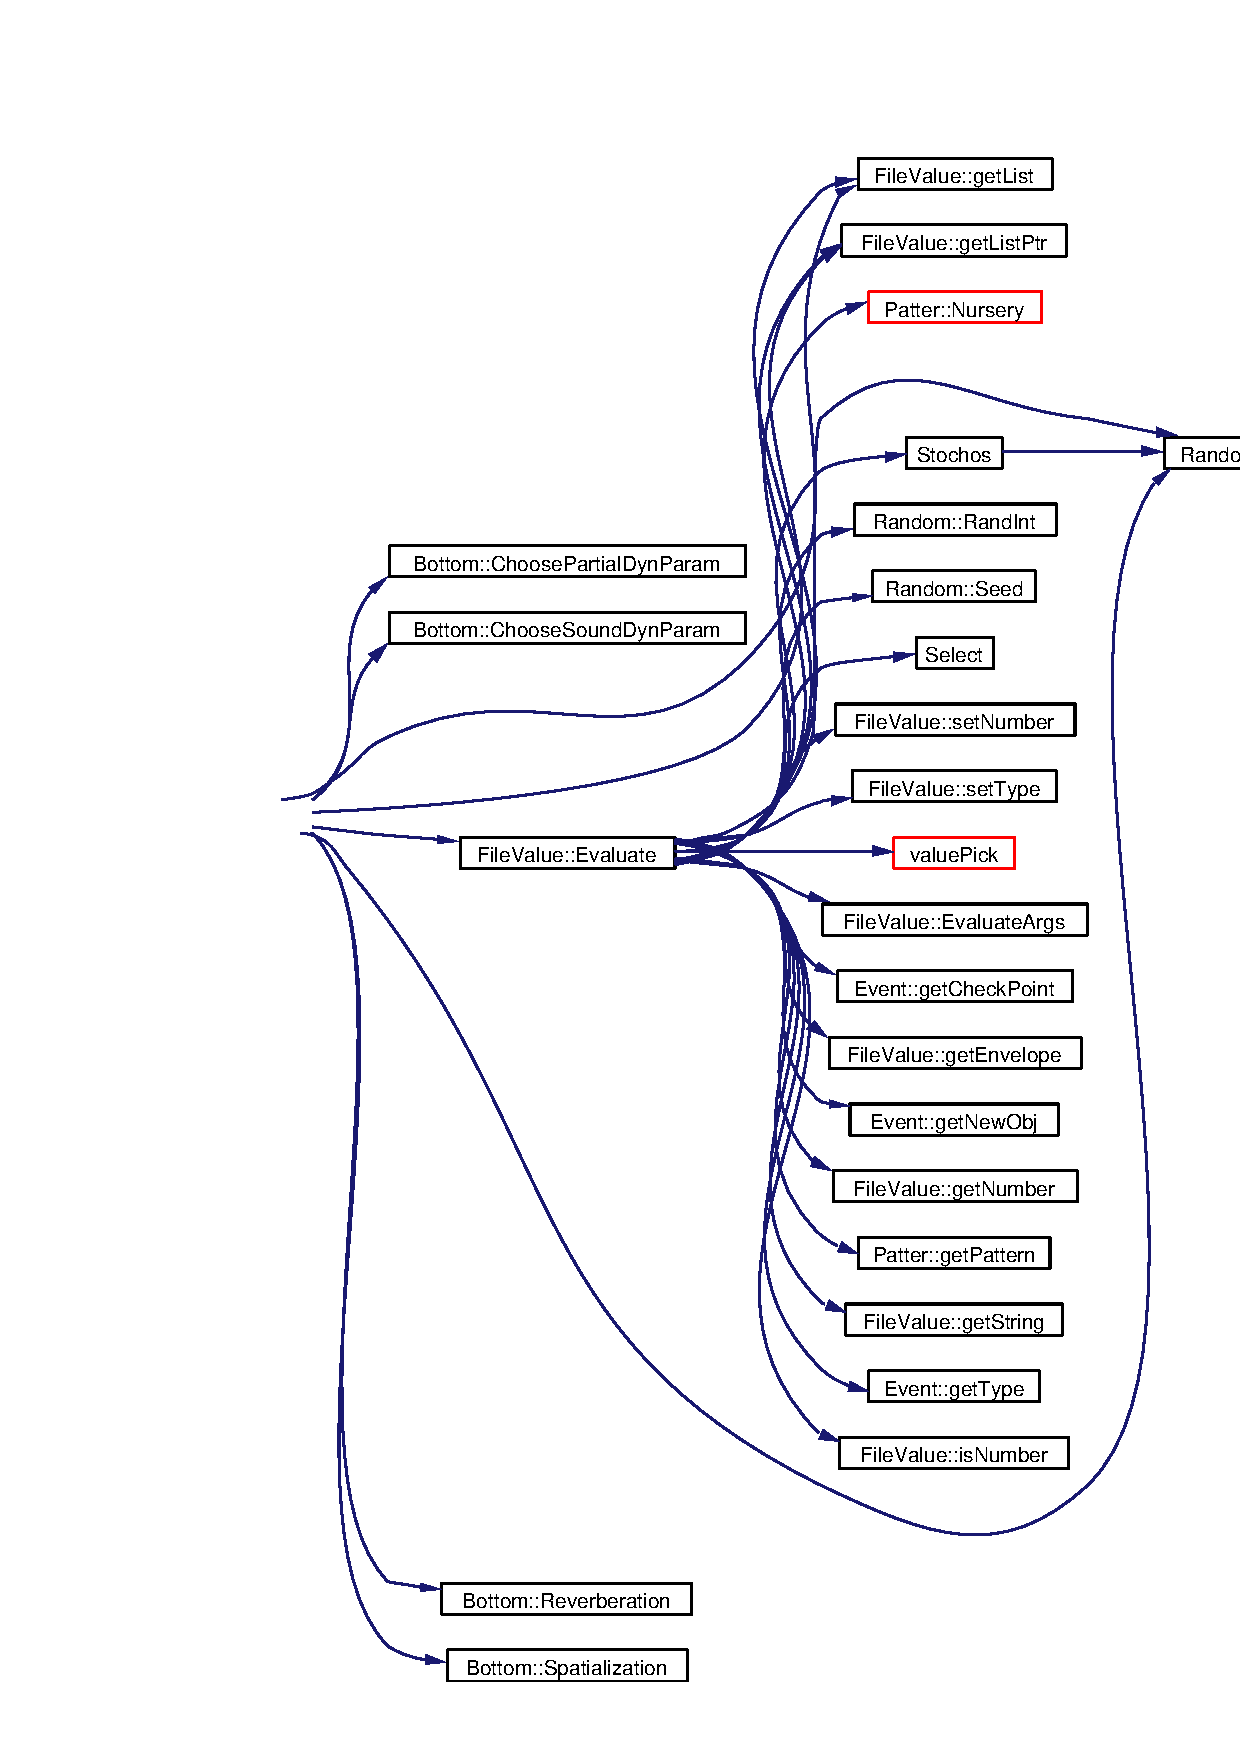
\includegraphics[width=325pt]{classBottom_a13_cgraph}
\end{center}
\end{figure}
\index{Bottom@{Bottom}!ChoosePartialDynParam@{ChoosePartialDynParam}}
\index{ChoosePartialDynParam@{ChoosePartialDynParam}!Bottom@{Bottom}}
\subsubsection{\setlength{\rightskip}{0pt plus 5cm}void Bottom::Choose\-Partial\-Dyn\-Param (Sound $\ast$ {\em s}, const char $\ast$ {\em modifier}, Envelope $\ast$ {\em env}, int {\em i})}\label{classBottom_a25}


FUNCTION: choosepartialdynparam INPUTS: Pointer to a sound Pointer to a const char containing the modifier information Pointer to an envelope Integer i representing the ith partial of a sound s

DESCRIPTION: This function sets the partial parameter specified in the modifier variable to what is contained in the envelope for a given partial of a sound s. 

Definition at line 672 of file bottom.cpp.

Referenced by build\-Sound(), and Modifiers().\index{Bottom@{Bottom}!ChooseSoundDynParam@{ChooseSoundDynParam}}
\index{ChooseSoundDynParam@{ChooseSoundDynParam}!Bottom@{Bottom}}
\subsubsection{\setlength{\rightskip}{0pt plus 5cm}void Bottom::Choose\-Sound\-Dyn\-Param (Sound $\ast$ {\em s}, const char $\ast$ {\em modifier}, Envelope $\ast$ {\em env})}\label{classBottom_a24}


FUNCTION: choosesounddynparam INPUTS: Pointer to a sound Pointer to a const char containing the modifier information Pointer to an envelope

DESCRIPTION: This function sets the partial parameter specified in the modifier variable to what is contained in the envelope for a given sound s. 

Definition at line 622 of file bottom.cpp.

References Event::check\-Point.

Referenced by build\-Sound(), and Modifiers().\index{Bottom@{Bottom}!clear@{clear}}
\index{clear@{clear}!Bottom@{Bottom}}
\subsubsection{\setlength{\rightskip}{0pt plus 5cm}void Bottom::clear ()\hspace{0.3cm}{\tt  [virtual]}}\label{classBottom_a5}


This function clears values of the Bottom object and to clear dynamic memory. 

Reimplemented from {\bf Event} {\rm (p.\,\pageref{classEvent_a12})}.

Reimplemented in {\bf Note} {\rm (p.\,\pageref{classNote_a14})}.

Definition at line 78 of file bottom.cpp.

References bottom\_\-abs\-Range, bottom\_\-amp\-Method, bottom\_\-amp\-Scale, bottom\_\-attenuation, bottom\_\-env\-Method, bottom\_\-factor, bottom\_\-freq\-Method, bottom\_\-freq\-Method2, bottom\_\-fundamental, bottom\_\-modifier, bottom\_\-new\-Object\-Method, bottom\_\-pat\-File, bottom\_\-rand\-Flag, bottom\_\-reverb\-Method, bottom\_\-rule, bottom\_\-select, bottom\_\-slope, bottom\_\-sound\-Method, bottom\_\-spat\-Method, Event::dur\-Array, Event::layer\-Dens, Event::max\-Types, Event::name\-Type, Event::objs\-In\-Layer, Event::prob\-Dur\-Array, Event::prob\-Sieve\-Array, Event::remain\-Objs, Event::star\-Tarray, Event::Test\-Name\-Type(), Event::the\-Name, and Event::types\-In\-Layer.

Here is the call graph for this function:\begin{figure}[H]
\begin{center}
\leavevmode
\includegraphics[width=140pt]{classBottom_a5_cgraph}
\end{center}
\end{figure}
\index{Bottom@{Bottom}!CreateNewObjects@{CreateNewObjects}}
\index{CreateNewObjects@{CreateNewObjects}!Bottom@{Bottom}}
\subsubsection{\setlength{\rightskip}{0pt plus 5cm}void Bottom::Create\-New\-Objects ()}\label{classBottom_a11}


This function uses a variety of methods to create new objects for the Bottom event. 

Reimplemented from {\bf Event} {\rm (p.\,\pageref{classEvent_a22})}.\index{Bottom@{Bottom}!CreatePartials@{CreatePartials}}
\index{CreatePartials@{CreatePartials}!Bottom@{Bottom}}
\subsubsection{\setlength{\rightskip}{0pt plus 5cm}void Bottom::Create\-Partials (Sound $\ast$ {\em s}, int {\em num\-Partials})}\label{classBottom_a17}


This function employs the LASS Partial class constructor and set\-Param function. \begin{Desc}
\item[Parameters:]
\begin{description}
\item[{\em s}]A sound \item[{\em num\-Partials}]The number of partials \end{description}
\end{Desc}


Definition at line 265 of file bottom.cpp.

Referenced by Spectrum().\index{Bottom@{Bottom}!Implement@{Implement}}
\index{Implement@{Implement}!Bottom@{Bottom}}
\subsubsection{\setlength{\rightskip}{0pt plus 5cm}void Bottom::Implement ()}\label{classBottom_a12}


This function chooses to implement a sound, a note, or a visual according to the type of output and the file used. \index{Bottom@{Bottom}!Loud@{Loud}}
\index{Loud@{Loud}!Bottom@{Bottom}}
\subsubsection{\setlength{\rightskip}{0pt plus 5cm}float Bottom::Loud (Sound $\ast$ {\em s}, double {\em check\-Point})}\label{classBottom_a22}


This function calculates the loudness of the given sound. \begin{Desc}
\item[Parameters:]
\begin{description}
\item[{\em s}]A sound \item[{\em check\-Point}]\end{description}
\end{Desc}
\begin{Desc}
\item[Returns:]The loudness of the sound \end{Desc}


Definition at line 493 of file bottom.cpp.

References Event::bottom\_\-loudness, File\-Value::Evaluate(), and File\-Value::get\-Number().

Here is the call graph for this function:\begin{figure}[H]
\begin{center}
\leavevmode
\includegraphics[width=363pt]{classBottom_a22_cgraph}
\end{center}
\end{figure}
\index{Bottom@{Bottom}!Modifiers@{Modifiers}}
\index{Modifiers@{Modifiers}!Bottom@{Bottom}}
\subsubsection{\setlength{\rightskip}{0pt plus 5cm}void Bottom::Modifiers (Sound $\ast$ {\em s}, int {\em num\-Partials}, double {\em check\-Point})}\label{classBottom_a23}


THIS FUNCTION NEEDS TO BE CONVERTED TO THE NEW CODE FUNCTION: modifiers INPUT: a pointer to a sound an integer containing the number of partials a double checkpoint

DESCRIPTION: 

Definition at line 524 of file bottom.cpp.

References bottom\_\-modifier, bottom\_\-select, Chance(), Choose\-Partial\-Dyn\-Param(), Choose\-Sound\-Dyn\-Param(), Envelope\-Builder(), envlib, File\-Value::get\-List\-Ptr(), File\-Value::get\-String(), and Read\-Compute\-Int().

Here is the call graph for this function:\begin{figure}[H]
\begin{center}
\leavevmode
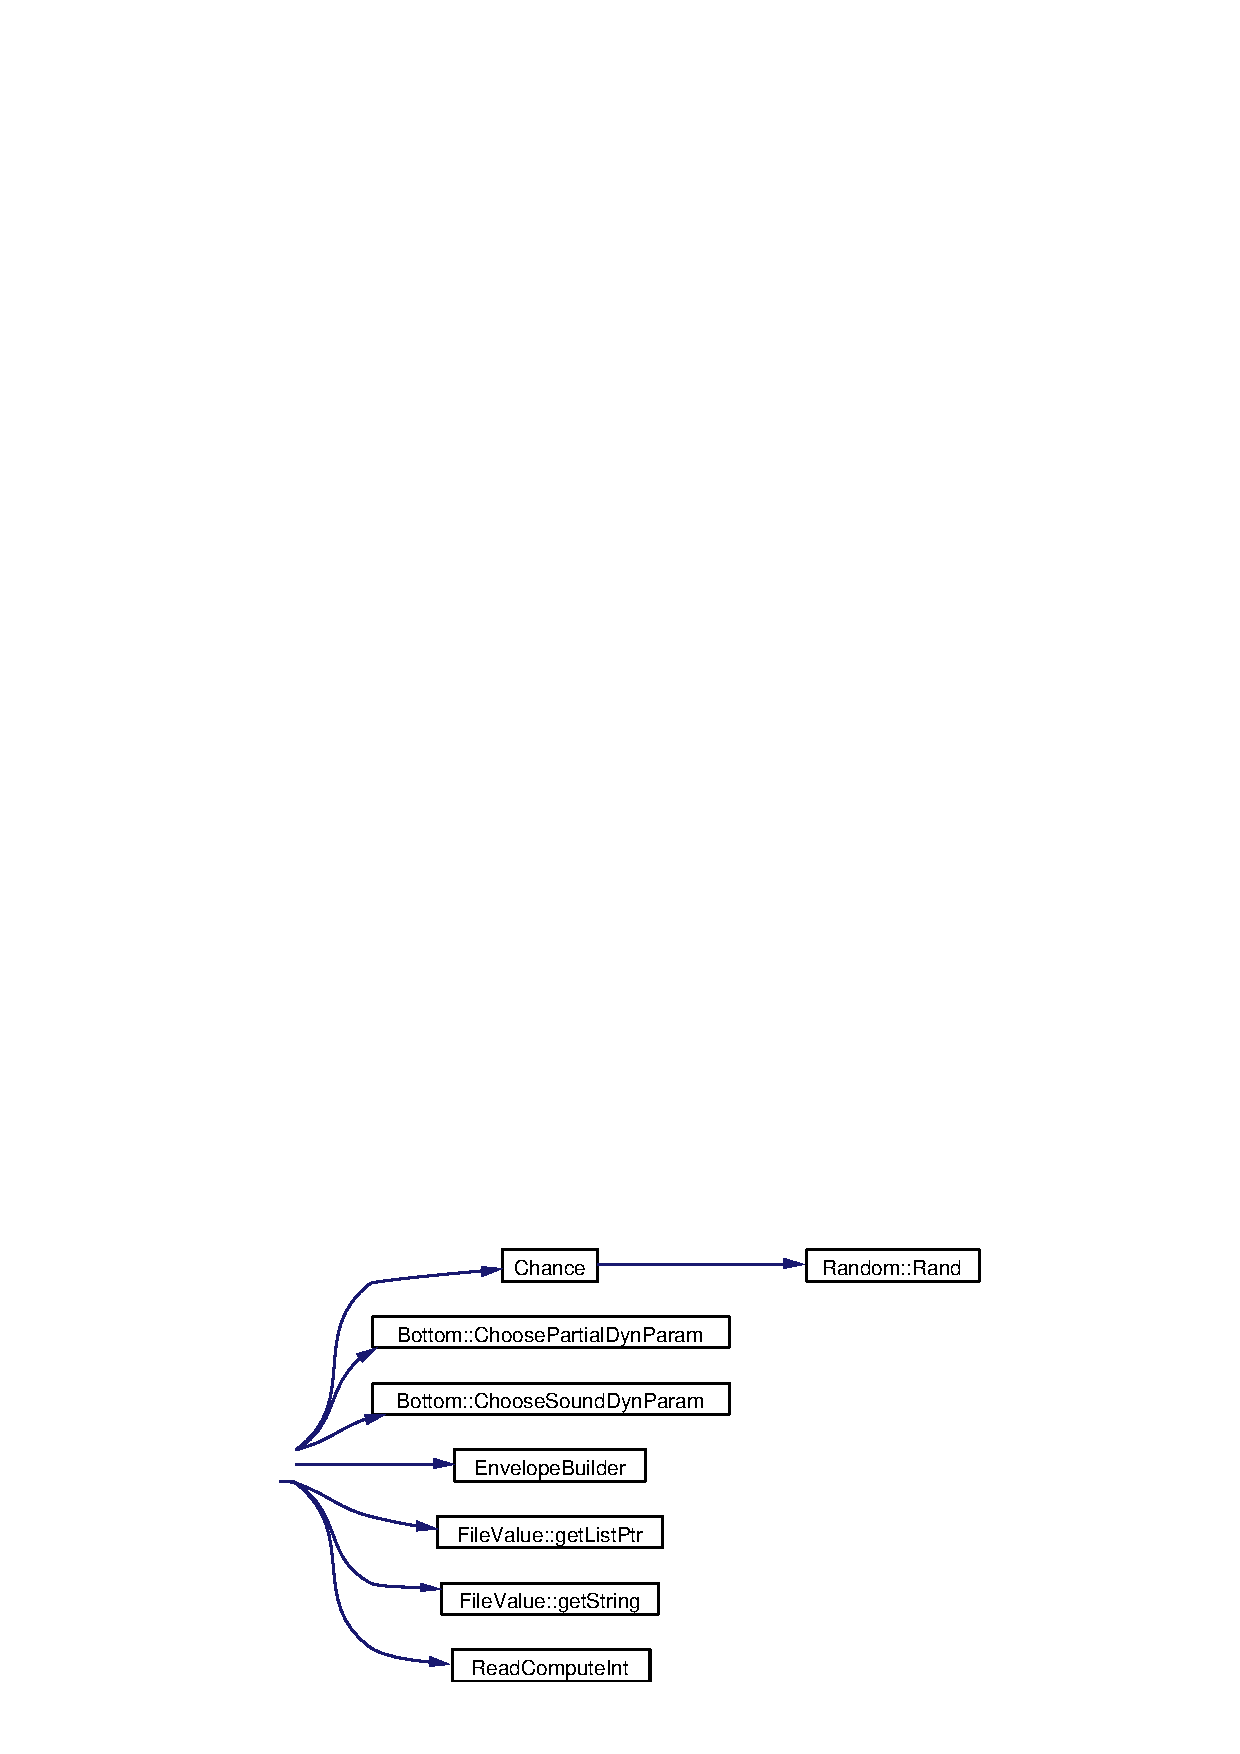
\includegraphics[width=239pt]{classBottom_a23_cgraph}
\end{center}
\end{figure}
\index{Bottom@{Bottom}!NumPart@{NumPart}}
\index{NumPart@{NumPart}!Bottom@{Bottom}}
\subsubsection{\setlength{\rightskip}{0pt plus 5cm}int Bottom::Num\-Part (float {\em freq})}\label{classBottom_a15}


This function determines how many partials a sound has by receiving the number of partials and then checking if any partial has a frequency higher than CEILING and discards those who have. \begin{Desc}
\item[Parameters:]
\begin{description}
\item[{\em freq}]\item[{\em num\-Partials}]\end{description}
\end{Desc}
\begin{Desc}
\item[Returns:]the number of partials a sound has \end{Desc}


Definition at line 201 of file bottom.cpp.

References CEILING, File\-Value::get\-Number(), sever, and Event::sound\_\-num\-Partials.

Referenced by Spectrum().

Here is the call graph for this function:\begin{figure}[H]
\begin{center}
\leavevmode
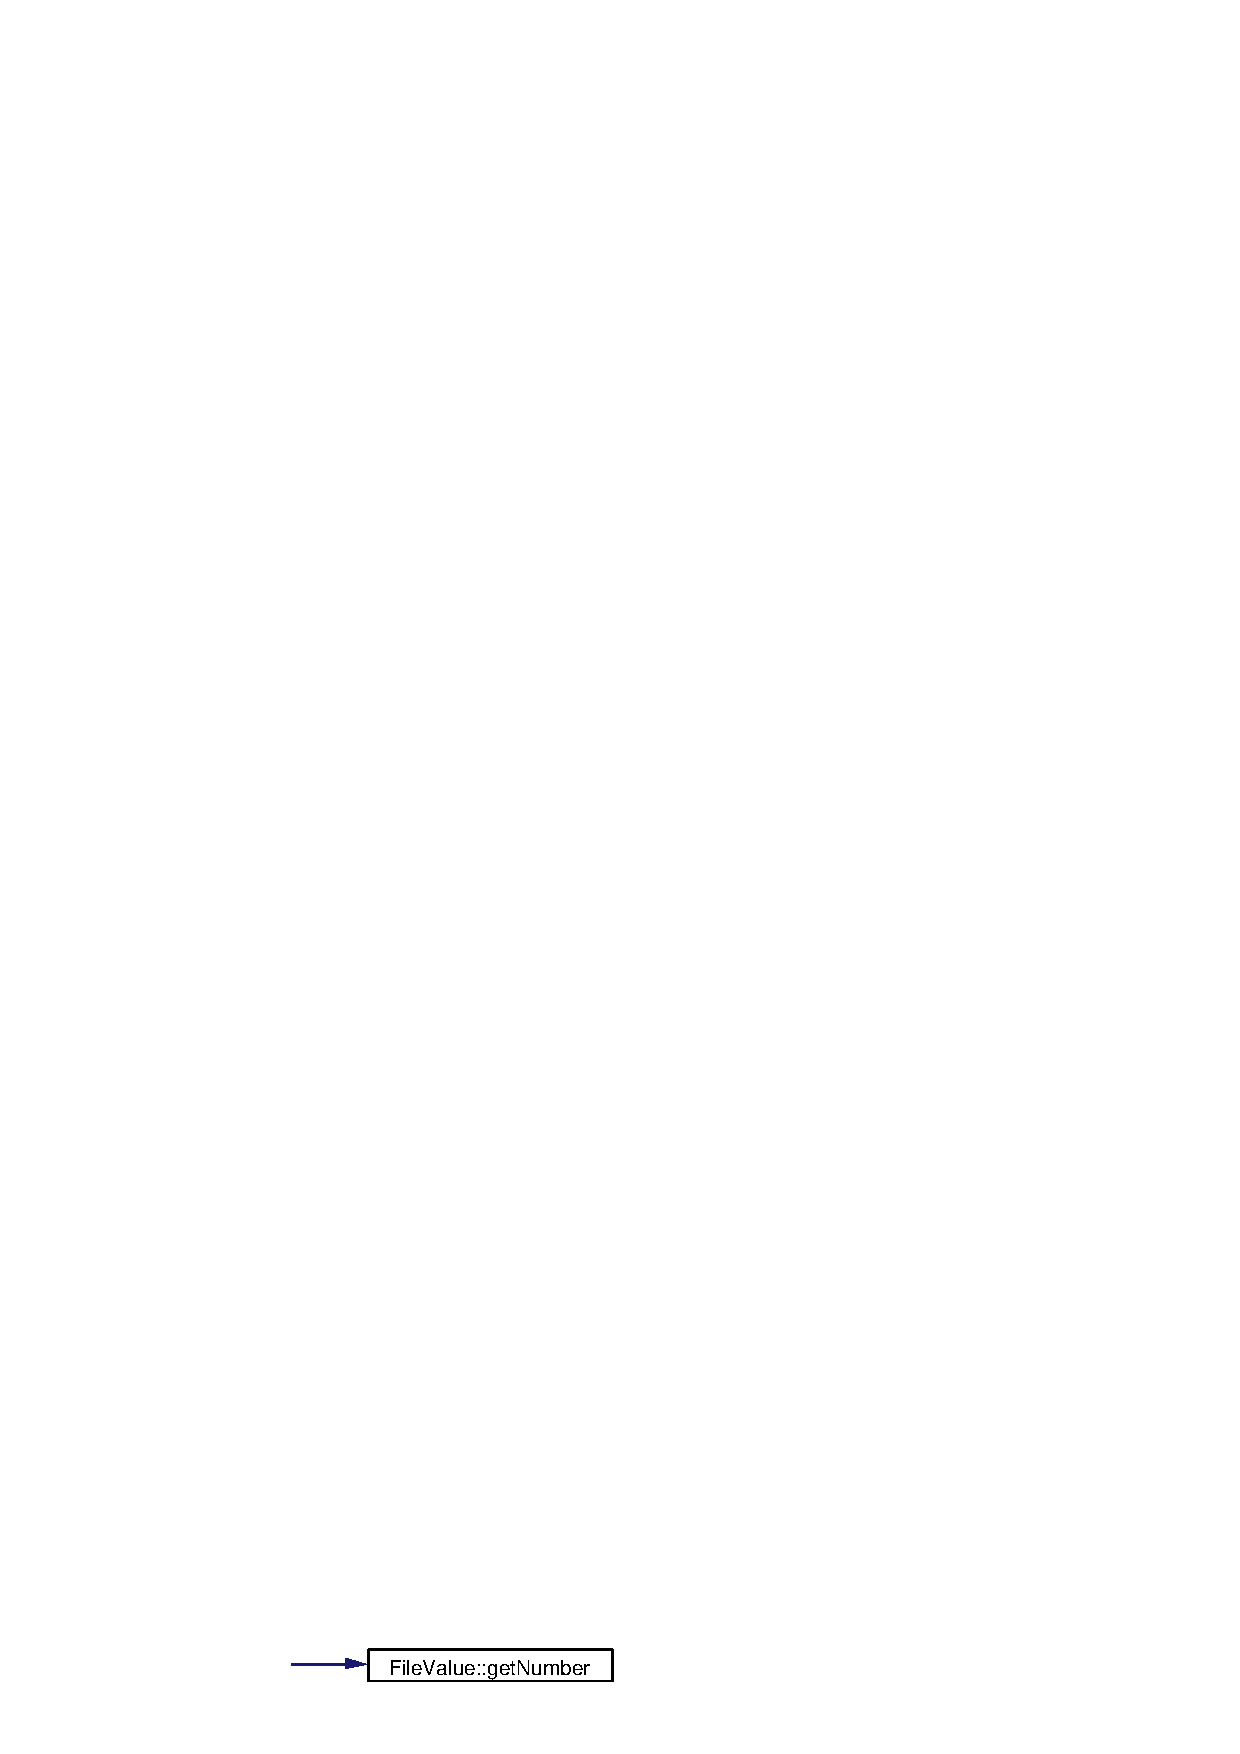
\includegraphics[width=151pt]{classBottom_a15_cgraph}
\end{center}
\end{figure}
\index{Bottom@{Bottom}!OneStep@{OneStep}}
\index{OneStep@{OneStep}!Bottom@{Bottom}}
\subsubsection{\setlength{\rightskip}{0pt plus 5cm}void Bottom::One\-Step (Sound $\ast$ {\em s}, double {\em check\-Point}, int {\em num\-Partials})}\label{classBottom_a19}


This function chooses an envelope for each partial and assigns it. \begin{Desc}
\item[Parameters:]
\begin{description}
\item[{\em s}]A sound \item[{\em check\-Point}]\item[{\em num\-Partials}]The number of partials \item[{\em sound\-File}]\end{description}
\end{Desc}


Definition at line 330 of file bottom.cpp.

References Choose\-Offset(), Envelope\-Builder(), Event::new\-Obj, and Event::type.

Referenced by Spectrum().

Here is the call graph for this function:\begin{figure}[H]
\begin{center}
\leavevmode
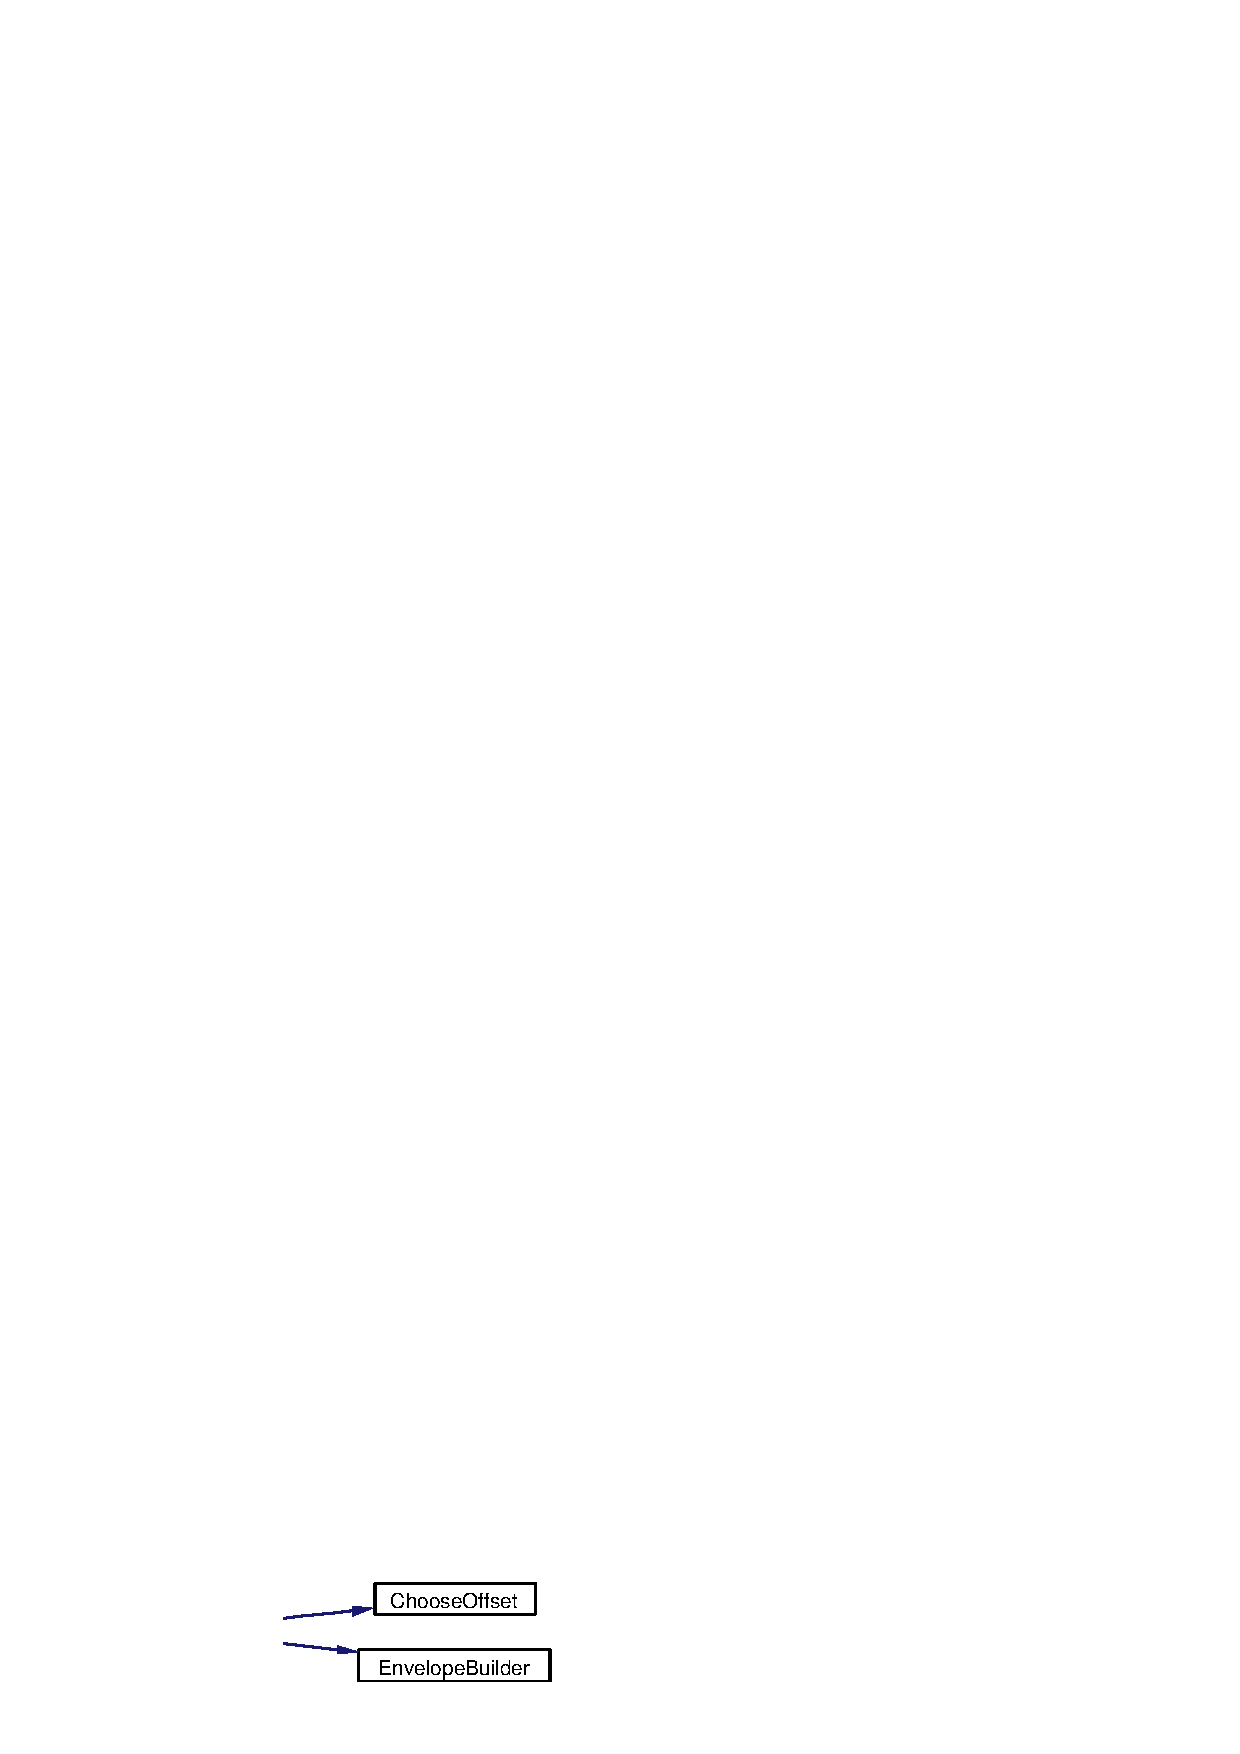
\includegraphics[width=136pt]{classBottom_a19_cgraph}
\end{center}
\end{figure}
\index{Bottom@{Bottom}!operator=@{operator=}}
\index{operator=@{operator=}!Bottom@{Bottom}}
\subsubsection{\setlength{\rightskip}{0pt plus 5cm}{\bf Bottom}\& Bottom::operator= (const {\bf Bottom} \& {\em orig\-Bottom})}\label{classBottom_a4}


This is an operator overload to define '=' as a call to the copy constructor. \begin{Desc}
\item[Parameters:]
\begin{description}
\item[{\em orig\-Bottom}]The Bottom to copy \end{description}
\end{Desc}
\begin{Desc}
\item[Returns:]A copy of orig\-Bottom \end{Desc}
\index{Bottom@{Bottom}!Print@{Print}}
\index{Print@{Print}!Bottom@{Bottom}}
\subsubsection{\setlength{\rightskip}{0pt plus 5cm}void Bottom::Print ()\hspace{0.3cm}{\tt  [virtual]}}\label{classBottom_a30}


FUNCTION: public: print

DESCRIPTION: Prints bottom id, name, start time and duration to outputfile 

Reimplemented from {\bf Event} {\rm (p.\,\pageref{classEvent_a57})}.

Definition at line 848 of file bottom.cpp.

References bottom\-ID, output\-File, Event::the\-Duration, Event::the\-Name, Event::the\-Start\-Time, and Event::u\-Per\-Sec.

Referenced by Note::Activate().\index{Bottom@{Bottom}!PrintSound@{PrintSound}}
\index{PrintSound@{PrintSound}!Bottom@{Bottom}}
\subsubsection{\setlength{\rightskip}{0pt plus 5cm}void Bottom::Print\-Sound (int {\em num\-Partials}, float {\em freq}, float {\em sones})}\label{classBottom_a31}


FUNCTION: printsound INPUT: Integer containing the number of partials Float containing the freq value Float containing the sones value

DESCRIPTION: Prints the sound id, start time, duration, type, freq, and sones of a sound 

Definition at line 871 of file bottom.cpp.

References Event::dur\-Sec, Event::obj\-ID, output\-File, Event::stime\-Sec, and Event::type.\index{Bottom@{Bottom}!Reverberation@{Reverberation}}
\index{Reverberation@{Reverberation}!Bottom@{Bottom}}
\subsubsection{\setlength{\rightskip}{0pt plus 5cm}void Bottom::Reverberation (Sound $\ast$ {\em s}, double {\em check\-Point}, string {\em method}, Envelope $\ast$ {\em chance}, float {\em room\-Size})}\label{classBottom_a29}


THIS FUNCTION IS OLD AND NEEDS TO BE UPDATED TO THE NEW CODE FUNCTION: reverberation INPUT: Pointer to a sound Double checkpoint String contain \char`\"{}room\_\-size\char`\"{}, \char`\"{}custom\char`\"{}, or \char`\"{}single\_\-partial\char`\"{} Pointer to an envelope Float roomsize

DESCRIPTION: Uses chance function and method to randomly create the reverberation for a sound 

Definition at line 779 of file bottom.cpp.

References bottom\_\-reverb\-Method, Chance(), and File\-Value::get\-String().

Here is the call graph for this function:\begin{figure}[H]
\begin{center}
\leavevmode
\includegraphics[width=216pt]{classBottom_a29_cgraph}
\end{center}
\end{figure}
\index{Bottom@{Bottom}!Reverberation@{Reverberation}}
\index{Reverberation@{Reverberation}!Bottom@{Bottom}}
\subsubsection{\setlength{\rightskip}{0pt plus 5cm}void Bottom::Reverberation (Sound $\ast$ {\em s}, double {\em check\-Point})}\label{classBottom_a28}




Referenced by build\-Sound().\index{Bottom@{Bottom}!Rules@{Rules}}
\index{Rules@{Rules}!Bottom@{Bottom}}
\subsubsection{\setlength{\rightskip}{0pt plus 5cm}void Bottom::Rules (int {\em num\-Partials}, float {\em amp\-Scale}[$\,$])}\label{classBottom_a21}


NOT DEFINED YET \begin{Desc}
\item[Parameters:]
\begin{description}
\item[{\em num\-Partials}]The number of partials \item[{\em amp\-Scale}]\end{description}
\end{Desc}


Definition at line 439 of file bottom.cpp.

References bottom\_\-amp\-Scale, bottom\_\-attenuation, bottom\_\-factor, bottom\_\-rand\-Flag, bottom\_\-rule, Exponential(), File\-Value::get\-Number(), File\-Value::get\-String(), Random::Rand(), Random::RAND\_\-SIGN, and sever.

Referenced by Three\-Step().

Here is the call graph for this function:\begin{figure}[H]
\begin{center}
\leavevmode
\includegraphics[width=142pt]{classBottom_a21_cgraph}
\end{center}
\end{figure}
\index{Bottom@{Bottom}!setDensity@{setDensity}}
\index{setDensity@{setDensity}!Bottom@{Bottom}}
\subsubsection{\setlength{\rightskip}{0pt plus 5cm}void Bottom::set\-Density (double {\em a\-Density})\hspace{0.3cm}{\tt  [virtual]}}\label{classBottom_a9}


This function sets the density of the Bottom event. \begin{Desc}
\item[Parameters:]
\begin{description}
\item[{\em a\-Density}]The amount to set the density to \end{description}
\end{Desc}


Reimplemented from {\bf Event} {\rm (p.\,\pageref{classEvent_a11})}.

Definition at line 175 of file bottom.cpp.

References bottom\-Density.

Referenced by Bottom().\index{Bottom@{Bottom}!setDuration@{setDuration}}
\index{setDuration@{setDuration}!Bottom@{Bottom}}
\subsubsection{\setlength{\rightskip}{0pt plus 5cm}void Bottom::set\-Duration (float {\em a\-Duration})\hspace{0.3cm}{\tt  [virtual]}}\label{classBottom_a8}


This function sets the duration of the Bottom event. \begin{Desc}
\item[Parameters:]
\begin{description}
\item[{\em a\-Duration}]The amount to set the duration to \end{description}
\end{Desc}


Reimplemented from {\bf Event} {\rm (p.\,\pageref{classEvent_a8})}.

Definition at line 166 of file bottom.cpp.

References bottom\-Duration.

Referenced by Bottom().\index{Bottom@{Bottom}!SetFrequency@{SetFrequency}}
\index{SetFrequency@{SetFrequency}!Bottom@{Bottom}}
\subsubsection{\setlength{\rightskip}{0pt plus 5cm}void Bottom::Set\-Frequency (Sound $\ast$ {\em s}, float {\em deviation}, float {\em base\-Freq}, int {\em num\-Partials})}\label{classBottom_a18}


This function assigns a frequency to each partial according to base\-Freq and the deviation (which is randomly selected as positive or negative). Individual frequencies are checked against the MINFREQ and CEILING (see {\bf define.h}{\rm (p.\,\pageref{define_8h})}) and set (applied to the sound object) with set\-Param (LASS). \begin{Desc}
\item[Parameters:]
\begin{description}
\item[{\em s}]A sound \item[{\em deviation}]The deviation \item[{\em base\-Freq}]The base frequency \item[{\em num\-Partials}]The number of partials \end{description}
\end{Desc}


Definition at line 291 of file bottom.cpp.

References CEILING, MINFREQ, and Random::Rand().

Referenced by Spectrum().

Here is the call graph for this function:\begin{figure}[H]
\begin{center}
\leavevmode
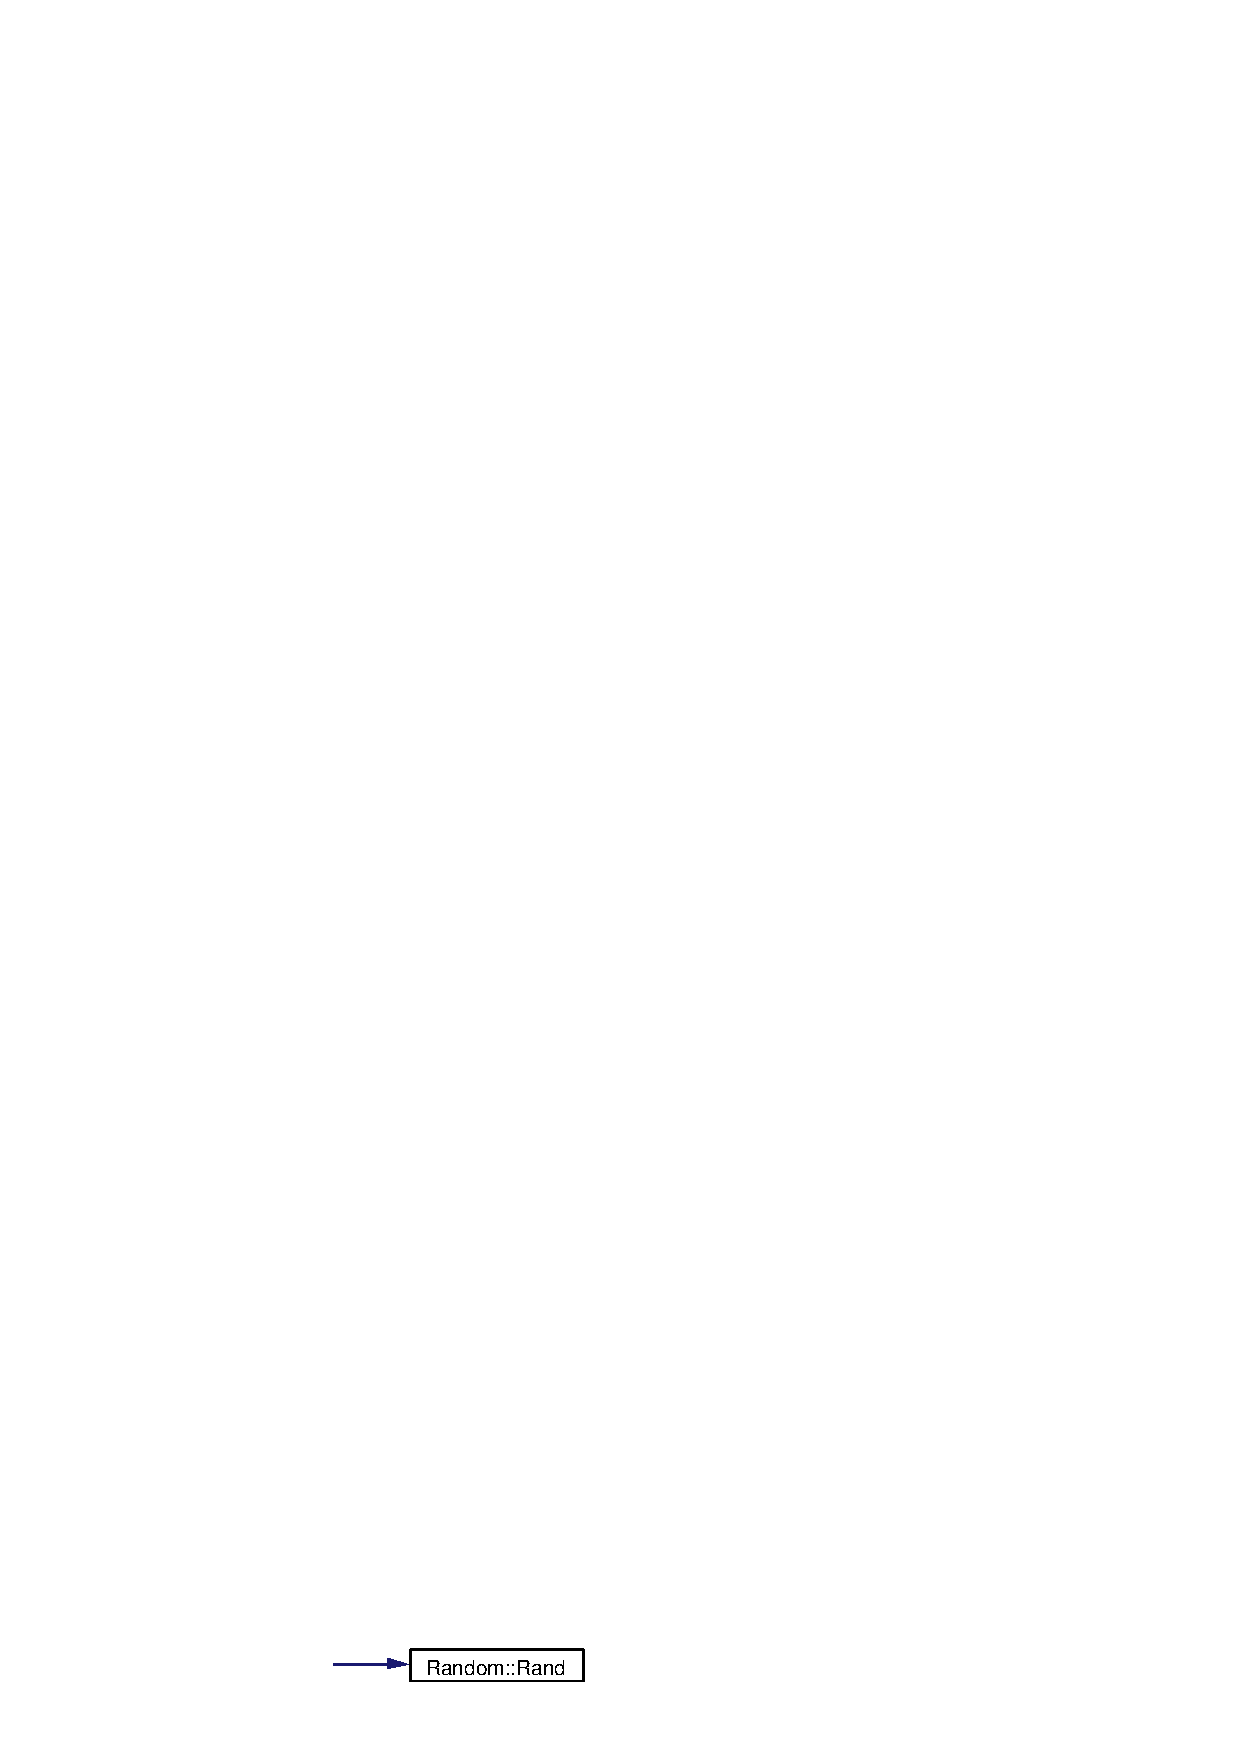
\includegraphics[width=144pt]{classBottom_a18_cgraph}
\end{center}
\end{figure}
\index{Bottom@{Bottom}!setName@{setName}}
\index{setName@{setName}!Bottom@{Bottom}}
\subsubsection{\setlength{\rightskip}{0pt plus 5cm}void Bottom::set\-Name (char $\ast$ {\em a\-Name})\hspace{0.3cm}{\tt  [virtual]}}\label{classBottom_a6}


This function sets the name of the Bottom event. \begin{Desc}
\item[Parameters:]
\begin{description}
\item[{\em a\-Name}]The name to set the bottom event to \end{description}
\end{Desc}


Reimplemented from {\bf Event} {\rm (p.\,\pageref{classEvent_a10})}.

Definition at line 142 of file bottom.cpp.

References bottom\-Name.

Referenced by Bottom().\index{Bottom@{Bottom}!setNumPartials@{setNumPartials}}
\index{setNumPartials@{setNumPartials}!Bottom@{Bottom}}
\subsubsection{\setlength{\rightskip}{0pt plus 5cm}void Bottom::set\-Num\-Partials (int {\em a\-Num\-Partials})}\label{classBottom_a10}


This function sets the number of partials of the Bottom {\bf Event}{\rm (p.\,\pageref{classEvent})} \begin{Desc}
\item[Parameters:]
\begin{description}
\item[{\em a\-Num\-Partials}]The numbers of partials \end{description}
\end{Desc}
\index{Bottom@{Bottom}!setStartTime@{setStartTime}}
\index{setStartTime@{setStartTime}!Bottom@{Bottom}}
\subsubsection{\setlength{\rightskip}{0pt plus 5cm}void Bottom::set\-Start\-Time (float {\em a\-Start\-Time})\hspace{0.3cm}{\tt  [virtual]}}\label{classBottom_a7}


This function sets the start time of the Bottom event. \begin{Desc}
\item[Parameters:]
\begin{description}
\item[{\em a\-Start\-Time}]The time to set the start time to \end{description}
\end{Desc}


Reimplemented from {\bf Event} {\rm (p.\,\pageref{classEvent_a7})}.

Definition at line 157 of file bottom.cpp.

References bottom\-Start\-Time.

Referenced by Bottom().\index{Bottom@{Bottom}!Spatialization@{Spatialization}}
\index{Spatialization@{Spatialization}!Bottom@{Bottom}}
\subsubsection{\setlength{\rightskip}{0pt plus 5cm}void Bottom::Spatialization (Sound $\ast$ {\em s}, double {\em check\-Point}, string {\em method}, Envelope $\ast$ {\em chance}, Envelope $\ast$ {\em pan})}\label{classBottom_a27}


NOTE: multi\_\-pan is unfinished. Think function is in process of being updated? FUNCTION: spatialization INPUT: Pointer to a sound Double checkpoint String containing the method Pointer to an envelope for chance Pointer to an envelope for pan

DESCRIPTION: Sets the spatialization of a sound according to method and random chance 

Definition at line 727 of file bottom.cpp.

References Chance(), Event::num\-Objs, and sever.

Here is the call graph for this function:\begin{figure}[H]
\begin{center}
\leavevmode
\includegraphics[width=185pt]{classBottom_a27_cgraph}
\end{center}
\end{figure}
\index{Bottom@{Bottom}!Spatialization@{Spatialization}}
\index{Spatialization@{Spatialization}!Bottom@{Bottom}}
\subsubsection{\setlength{\rightskip}{0pt plus 5cm}void Bottom::Spatialization (Sound $\ast$ {\em s}, double {\em check\-Point})}\label{classBottom_a26}




Referenced by build\-Sound().\index{Bottom@{Bottom}!Spectrum@{Spectrum}}
\index{Spectrum@{Spectrum}!Bottom@{Bottom}}
\subsubsection{\setlength{\rightskip}{0pt plus 5cm}int Bottom::Spectrum (Sound $\ast$ {\em s}, float {\em freq})}\label{classBottom_a16}


NOT YET DEFINED \begin{Desc}
\item[Parameters:]
\begin{description}
\item[{\em s}]A sound \item[{\em freq}]\end{description}
\end{Desc}


Definition at line 230 of file bottom.cpp.

References bottom\_\-sound\-Method, Event::check\-Point, Create\-Partials(), File\-Value::get\-Number(), File\-Value::get\-String(), Num\-Part(), One\-Step(), Set\-Frequency(), sever, Event::sound\_\-deviation, and Three\-Step().

Here is the call graph for this function:\begin{figure}[H]
\begin{center}
\leavevmode
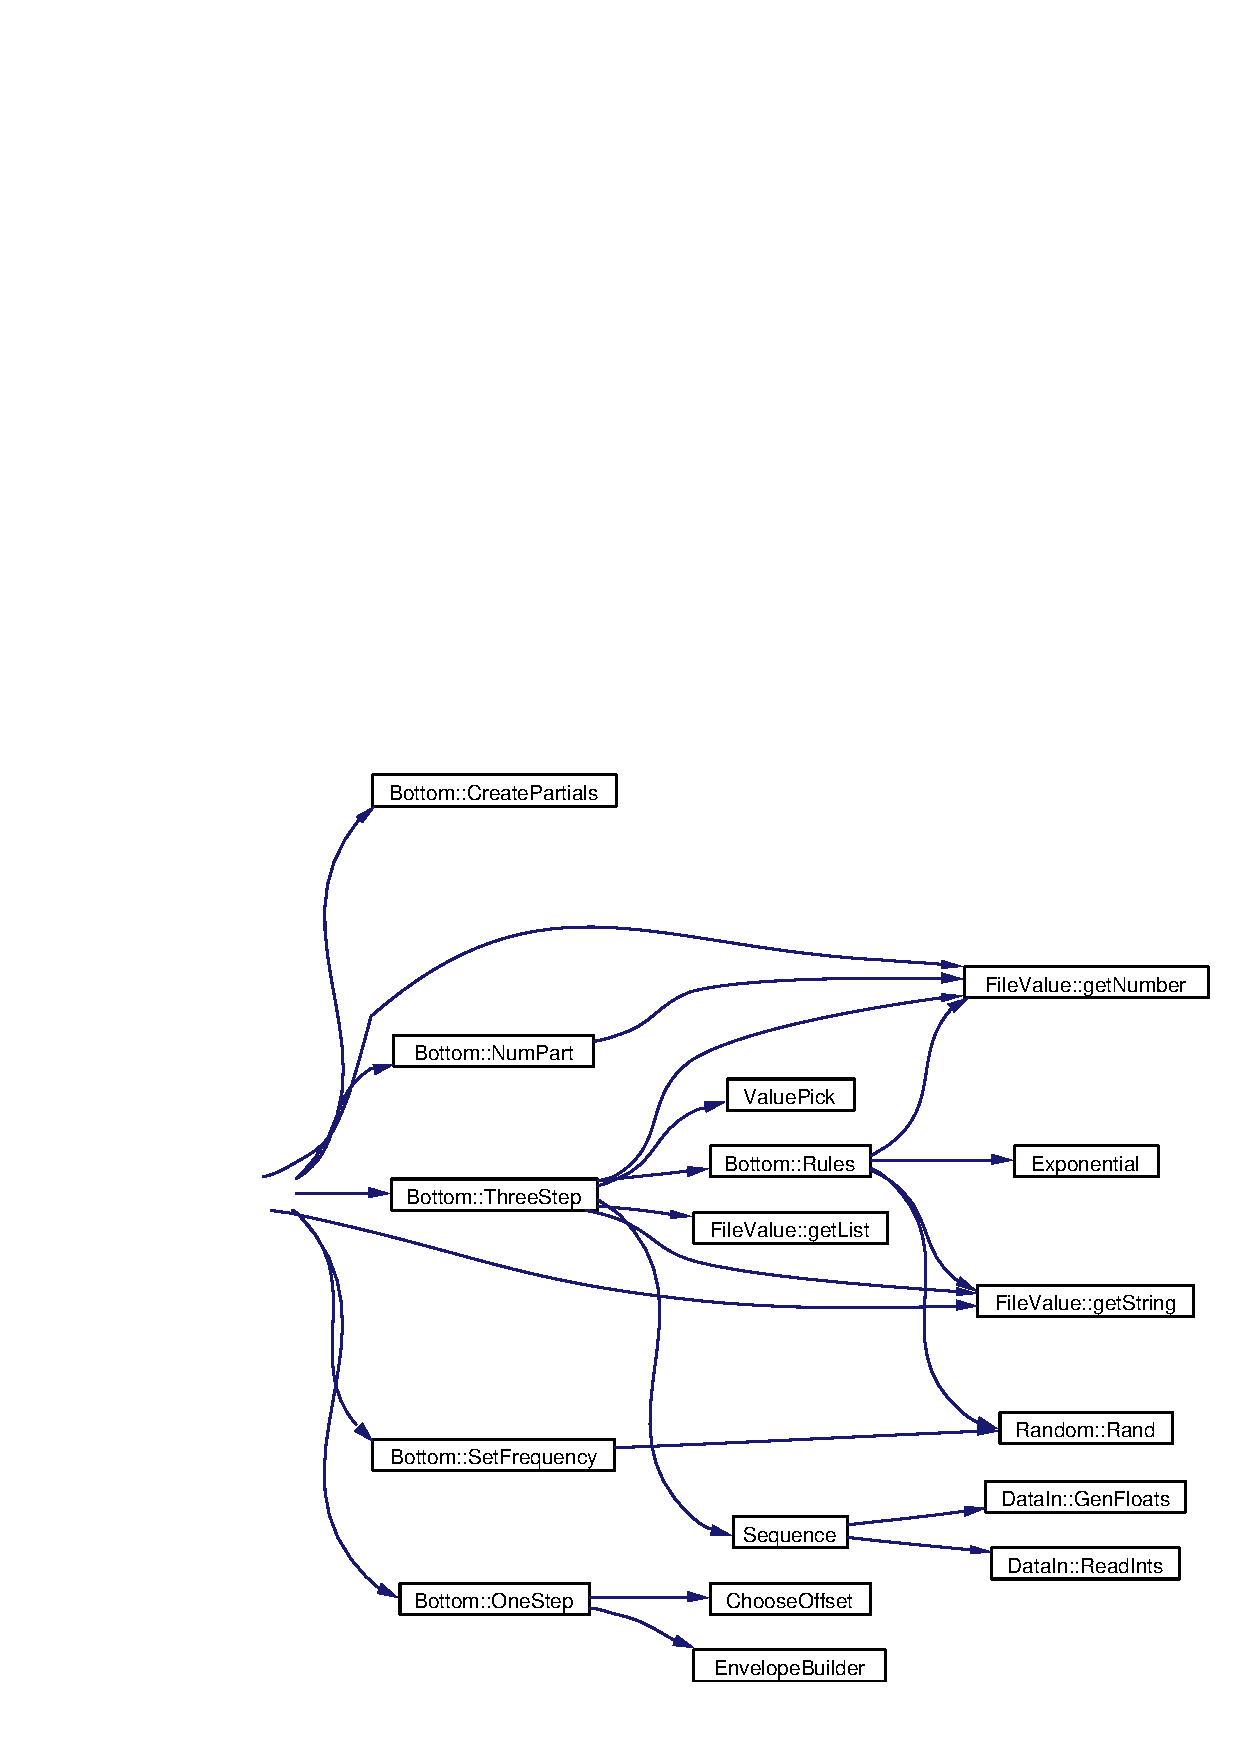
\includegraphics[width=294pt]{classBottom_a16_cgraph}
\end{center}
\end{figure}
\index{Bottom@{Bottom}!ThreeStep@{ThreeStep}}
\index{ThreeStep@{ThreeStep}!Bottom@{Bottom}}
\subsubsection{\setlength{\rightskip}{0pt plus 5cm}void Bottom::Three\-Step (Sound $\ast$ {\em s}, double {\em check\-Point}, int {\em num\-Partials})}\label{classBottom_a20}


NOT DEFINED YET \begin{Desc}
\item[Parameters:]
\begin{description}
\item[{\em s}]A sound \item[{\em check\-Point}]\item[{\em num\-Partials}]The number of partials \end{description}
\end{Desc}


Definition at line 362 of file bottom.cpp.

References bottom\_\-abs\-Range, bottom\_\-amp\-Method, bottom\_\-amp\-Scale, bottom\_\-env\-Method, envlib, File\-Value::get\-List(), File\-Value::get\-Number(), File\-Value::get\-String(), Rules(), Sequence(), sever, and Value\-Pick().

Referenced by Spectrum().

Here is the call graph for this function:\begin{figure}[H]
\begin{center}
\leavevmode
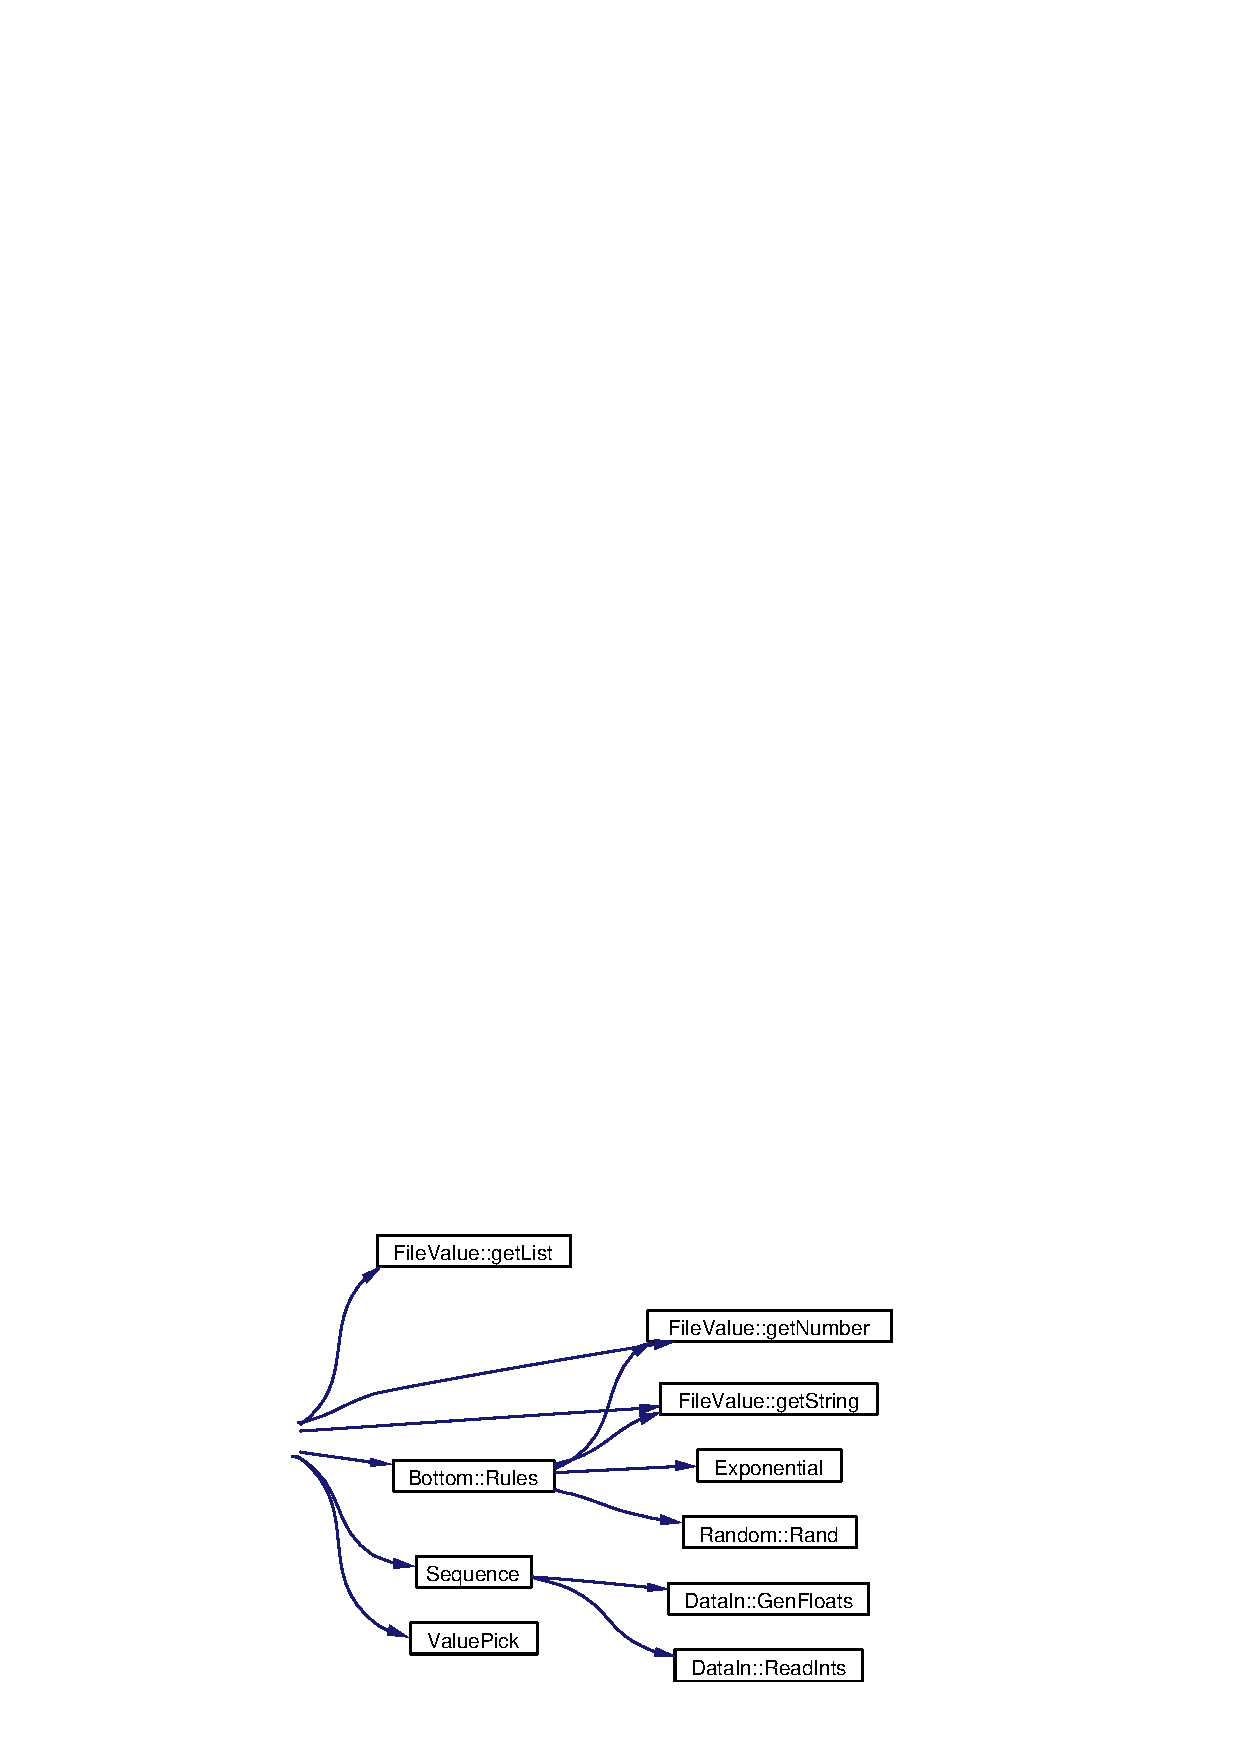
\includegraphics[width=218pt]{classBottom_a20_cgraph}
\end{center}
\end{figure}


\subsection{Member Data Documentation}
\index{Bottom@{Bottom}!bottom_absRange@{bottom\_\-absRange}}
\index{bottom_absRange@{bottom\_\-absRange}!Bottom@{Bottom}}
\subsubsection{\setlength{\rightskip}{0pt plus 5cm}{\bf File\-Value}$\ast$ {\bf Bottom::bottom\_\-abs\-Range}}\label{classBottom_o4}




Definition at line 302 of file bottom.h.

Referenced by clear(), and Three\-Step().\index{Bottom@{Bottom}!bottom_ampMethod@{bottom\_\-ampMethod}}
\index{bottom_ampMethod@{bottom\_\-ampMethod}!Bottom@{Bottom}}
\subsubsection{\setlength{\rightskip}{0pt plus 5cm}{\bf File\-Value}$\ast$ {\bf Bottom::bottom\_\-amp\-Method}}\label{classBottom_o9}




Definition at line 307 of file bottom.h.

Referenced by clear(), and Three\-Step().\index{Bottom@{Bottom}!bottom_ampScale@{bottom\_\-ampScale}}
\index{bottom_ampScale@{bottom\_\-ampScale}!Bottom@{Bottom}}
\subsubsection{\setlength{\rightskip}{0pt plus 5cm}{\bf File\-Value}$\ast$ {\bf Bottom::bottom\_\-amp\-Scale}}\label{classBottom_o12}




Definition at line 310 of file bottom.h.

Referenced by clear(), Rules(), and Three\-Step().\index{Bottom@{Bottom}!bottom_attenuation@{bottom\_\-attenuation}}
\index{bottom_attenuation@{bottom\_\-attenuation}!Bottom@{Bottom}}
\subsubsection{\setlength{\rightskip}{0pt plus 5cm}{\bf File\-Value}$\ast$ {\bf Bottom::bottom\_\-attenuation}}\label{classBottom_o14}




Definition at line 312 of file bottom.h.

Referenced by clear(), and Rules().\index{Bottom@{Bottom}!bottom_envMethod@{bottom\_\-envMethod}}
\index{bottom_envMethod@{bottom\_\-envMethod}!Bottom@{Bottom}}
\subsubsection{\setlength{\rightskip}{0pt plus 5cm}{\bf File\-Value}$\ast$ {\bf Bottom::bottom\_\-env\-Method}}\label{classBottom_o8}




Definition at line 306 of file bottom.h.

Referenced by clear(), and Three\-Step().\index{Bottom@{Bottom}!bottom_factor@{bottom\_\-factor}}
\index{bottom_factor@{bottom\_\-factor}!Bottom@{Bottom}}
\subsubsection{\setlength{\rightskip}{0pt plus 5cm}{\bf File\-Value}$\ast$ {\bf Bottom::bottom\_\-factor}}\label{classBottom_o13}




Definition at line 311 of file bottom.h.

Referenced by clear(), and Rules().\index{Bottom@{Bottom}!bottom_freqMethod@{bottom\_\-freqMethod}}
\index{bottom_freqMethod@{bottom\_\-freqMethod}!Bottom@{Bottom}}
\subsubsection{\setlength{\rightskip}{0pt plus 5cm}{\bf File\-Value}$\ast$ {\bf Bottom::bottom\_\-freq\-Method}}\label{classBottom_o2}




Definition at line 300 of file bottom.h.

Referenced by clear().\index{Bottom@{Bottom}!bottom_freqMethod2@{bottom\_\-freqMethod2}}
\index{bottom_freqMethod2@{bottom\_\-freqMethod2}!Bottom@{Bottom}}
\subsubsection{\setlength{\rightskip}{0pt plus 5cm}{\bf File\-Value}$\ast$ {\bf Bottom::bottom\_\-freq\-Method2}}\label{classBottom_o3}




Definition at line 301 of file bottom.h.

Referenced by clear().\index{Bottom@{Bottom}!bottom_fundamental@{bottom\_\-fundamental}}
\index{bottom_fundamental@{bottom\_\-fundamental}!Bottom@{Bottom}}
\subsubsection{\setlength{\rightskip}{0pt plus 5cm}{\bf File\-Value}$\ast$ {\bf Bottom::bottom\_\-fundamental}}\label{classBottom_o6}




Definition at line 304 of file bottom.h.

Referenced by clear().\index{Bottom@{Bottom}!bottom_modifier@{bottom\_\-modifier}}
\index{bottom_modifier@{bottom\_\-modifier}!Bottom@{Bottom}}
\subsubsection{\setlength{\rightskip}{0pt plus 5cm}{\bf File\-Value}$\ast$ {\bf Bottom::bottom\_\-modifier}}\label{classBottom_o15}




Definition at line 313 of file bottom.h.

Referenced by clear(), and Modifiers().\index{Bottom@{Bottom}!bottom_newObjectMethod@{bottom\_\-newObjectMethod}}
\index{bottom_newObjectMethod@{bottom\_\-newObjectMethod}!Bottom@{Bottom}}
\subsubsection{\setlength{\rightskip}{0pt plus 5cm}{\bf File\-Value}$\ast$ {\bf Bottom::bottom\_\-new\-Object\-Method}}\label{classBottom_o0}




Definition at line 298 of file bottom.h.

Referenced by clear().\index{Bottom@{Bottom}!bottom_patFile@{bottom\_\-patFile}}
\index{bottom_patFile@{bottom\_\-patFile}!Bottom@{Bottom}}
\subsubsection{\setlength{\rightskip}{0pt plus 5cm}{\bf File\-Value}$\ast$ {\bf Bottom::bottom\_\-pat\-File}}\label{classBottom_o5}




Definition at line 303 of file bottom.h.

Referenced by clear().\index{Bottom@{Bottom}!bottom_randFlag@{bottom\_\-randFlag}}
\index{bottom_randFlag@{bottom\_\-randFlag}!Bottom@{Bottom}}
\subsubsection{\setlength{\rightskip}{0pt plus 5cm}{\bf File\-Value}$\ast$ {\bf Bottom::bottom\_\-rand\-Flag}}\label{classBottom_o11}




Definition at line 309 of file bottom.h.

Referenced by clear(), and Rules().\index{Bottom@{Bottom}!bottom_reverbMethod@{bottom\_\-reverbMethod}}
\index{bottom_reverbMethod@{bottom\_\-reverbMethod}!Bottom@{Bottom}}
\subsubsection{\setlength{\rightskip}{0pt plus 5cm}{\bf File\-Value}$\ast$ {\bf Bottom::bottom\_\-reverb\-Method}}\label{classBottom_o18}




Definition at line 316 of file bottom.h.

Referenced by clear(), and Reverberation().\index{Bottom@{Bottom}!bottom_rule@{bottom\_\-rule}}
\index{bottom_rule@{bottom\_\-rule}!Bottom@{Bottom}}
\subsubsection{\setlength{\rightskip}{0pt plus 5cm}{\bf File\-Value}$\ast$ {\bf Bottom::bottom\_\-rule}}\label{classBottom_o10}




Definition at line 308 of file bottom.h.

Referenced by clear(), and Rules().\index{Bottom@{Bottom}!bottom_select@{bottom\_\-select}}
\index{bottom_select@{bottom\_\-select}!Bottom@{Bottom}}
\subsubsection{\setlength{\rightskip}{0pt plus 5cm}{\bf File\-Value}$\ast$ {\bf Bottom::bottom\_\-select}}\label{classBottom_o16}




Definition at line 314 of file bottom.h.

Referenced by clear(), and Modifiers().\index{Bottom@{Bottom}!bottom_slope@{bottom\_\-slope}}
\index{bottom_slope@{bottom\_\-slope}!Bottom@{Bottom}}
\subsubsection{\setlength{\rightskip}{0pt plus 5cm}{\bf File\-Value}$\ast$ {\bf Bottom::bottom\_\-slope}}\label{classBottom_o1}




Definition at line 299 of file bottom.h.

Referenced by clear().\index{Bottom@{Bottom}!bottom_soundMethod@{bottom\_\-soundMethod}}
\index{bottom_soundMethod@{bottom\_\-soundMethod}!Bottom@{Bottom}}
\subsubsection{\setlength{\rightskip}{0pt plus 5cm}{\bf File\-Value}$\ast$ {\bf Bottom::bottom\_\-sound\-Method}}\label{classBottom_o7}




Definition at line 305 of file bottom.h.

Referenced by clear(), and Spectrum().\index{Bottom@{Bottom}!bottom_spatMethod@{bottom\_\-spatMethod}}
\index{bottom_spatMethod@{bottom\_\-spatMethod}!Bottom@{Bottom}}
\subsubsection{\setlength{\rightskip}{0pt plus 5cm}{\bf File\-Value}$\ast$ {\bf Bottom::bottom\_\-spat\-Method}}\label{classBottom_o17}




Definition at line 315 of file bottom.h.

Referenced by clear().\index{Bottom@{Bottom}!bottomDensity@{bottomDensity}}
\index{bottomDensity@{bottomDensity}!Bottom@{Bottom}}
\subsubsection{\setlength{\rightskip}{0pt plus 5cm}double {\bf Bottom::bottom\-Density}\hspace{0.3cm}{\tt  [private]}}\label{classBottom_r0}


This is a double to hold the density 

Definition at line 56 of file bottom.h.

Referenced by set\-Density().\index{Bottom@{Bottom}!bottomDuration@{bottomDuration}}
\index{bottomDuration@{bottomDuration}!Bottom@{Bottom}}
\subsubsection{\setlength{\rightskip}{0pt plus 5cm}float {\bf Bottom::bottom\-Duration}\hspace{0.3cm}{\tt  [protected]}}\label{classBottom_p2}




Definition at line 336 of file bottom.h.

Referenced by set\-Duration().\index{Bottom@{Bottom}!bottomName@{bottomName}}
\index{bottomName@{bottomName}!Bottom@{Bottom}}
\subsubsection{\setlength{\rightskip}{0pt plus 5cm}char$\ast$ {\bf Bottom::bottom\-Name}\hspace{0.3cm}{\tt  [protected]}}\label{classBottom_p0}




Definition at line 326 of file bottom.h.

Referenced by set\-Name().\index{Bottom@{Bottom}!bottomNumPartials@{bottomNumPartials}}
\index{bottomNumPartials@{bottomNumPartials}!Bottom@{Bottom}}
\subsubsection{\setlength{\rightskip}{0pt plus 5cm}int {\bf Bottom::bottom\-Num\-Partials}\hspace{0.3cm}{\tt  [protected]}}\label{classBottom_p4}




Definition at line 346 of file bottom.h.\index{Bottom@{Bottom}!bottomStartTime@{bottomStartTime}}
\index{bottomStartTime@{bottomStartTime}!Bottom@{Bottom}}
\subsubsection{\setlength{\rightskip}{0pt plus 5cm}float {\bf Bottom::bottom\-Start\-Time}\hspace{0.3cm}{\tt  [protected]}}\label{classBottom_p1}




Definition at line 331 of file bottom.h.

Referenced by build\-Note(), and set\-Start\-Time().\index{Bottom@{Bottom}!bottomType@{bottomType}}
\index{bottomType@{bottomType}!Bottom@{Bottom}}
\subsubsection{\setlength{\rightskip}{0pt plus 5cm}int {\bf Bottom::bottom\-Type}\hspace{0.3cm}{\tt  [protected]}}\label{classBottom_p3}




Definition at line 341 of file bottom.h.

Referenced by Bottom().

The documentation for this class was generated from the following files:\begin{CompactItemize}
\item 
{\bf bottom.h}\item 
{\bf bottom.cpp}\end{CompactItemize}
